


Стрімкий розвиток інформаційних технологій та їх глибока інтеграція в усі сфери життя сучасного суспільства актуалізує проблему навчання учнів закладів загальної середньої освіти основам інформаційної безпеки. Цифрова трансформація освітнього процесу, масовий перехід на дистанційне навчання під час пандемії COVID-19, а також зростання кіберзагроз створюють нові виклики для педагогічної спільноти.

З метою визначення сучасного стану досліджень у галузі навчання інформаційній безпеці учнів було проведено комплексний бібліографічний аналіз наукових публікацій, представлених у науково-метричній базі Scopus. Пошук здійснювався за запитом: \textit{(``learning'' OR ``education'') AND (``information security'' OR ``Cybersecurity'') AND ``school''}, що дав змогу ідентифікувати 585 релевантних публікацій.

Для аналізу та візуалізації бібліографічних даних було використано програмне забезпечення VOSviewer /cite{VOSviewer}, яке надає інструменти для створення карт відповідності ключових слів та виявляти тематичні кластери в масиві наукових публікацій. Аналіз проводився за такими параметрами:
\begin{itemize}
    \item тип аналізу: відповідність ключових слів (co-occurrence);
    \item одиниця аналізу: усі ключові слова (all keywords);
    \item метод підрахунку: повний підрахунок (full counting);
    \item мінімальна кількість зустрічей ключового слова: 10.
\end{itemize}

З початкових 3407 ключових слів після застосування порогового значення було відібрано 71 термін, які сформували основу для кластерного аналізу.


Аналіз географічного розподілу публікацій виявив домінування англомовних країн у дослідженнях з навчання інформаційній безпеці в школах. Країни, які є лідерами за кількістю публікацій, зазначені в таблиці~\ref{leaders}

\begin{table}[h] 
\centering
\caption{Географічний розподіл публікацій з навчання інформаційній безпеці.}
\label{leaders}
\begin{tabular}{|l|c|c|c|}
\hline
\textbf{Країна} & \textbf{Документи} & \textbf{Цитування} & \textbf{Сила зв'язків} \\
\hline
США & 215 & 1285 & 17 \\
Австралія & 10 & 102 & 11 \\
Велика Британія & 24 & 238 & 9 \\
Канада & 7 & 54 & 7 \\
Південна Африка & 14 & 80 & 7 \\
Німеччина & 8 & 23 & 6 \\
Індія & 9 & 71 & 6 \\
\hline
\end{tabular}
\end{table}


Кластерний аналіз дав змогу виділити п'ять основних тематичних напрямів досліджень у галузі навчання інформаційній безпеці учнів (рис.~\ref{VOSmap}):

\begin{figure}[h]
    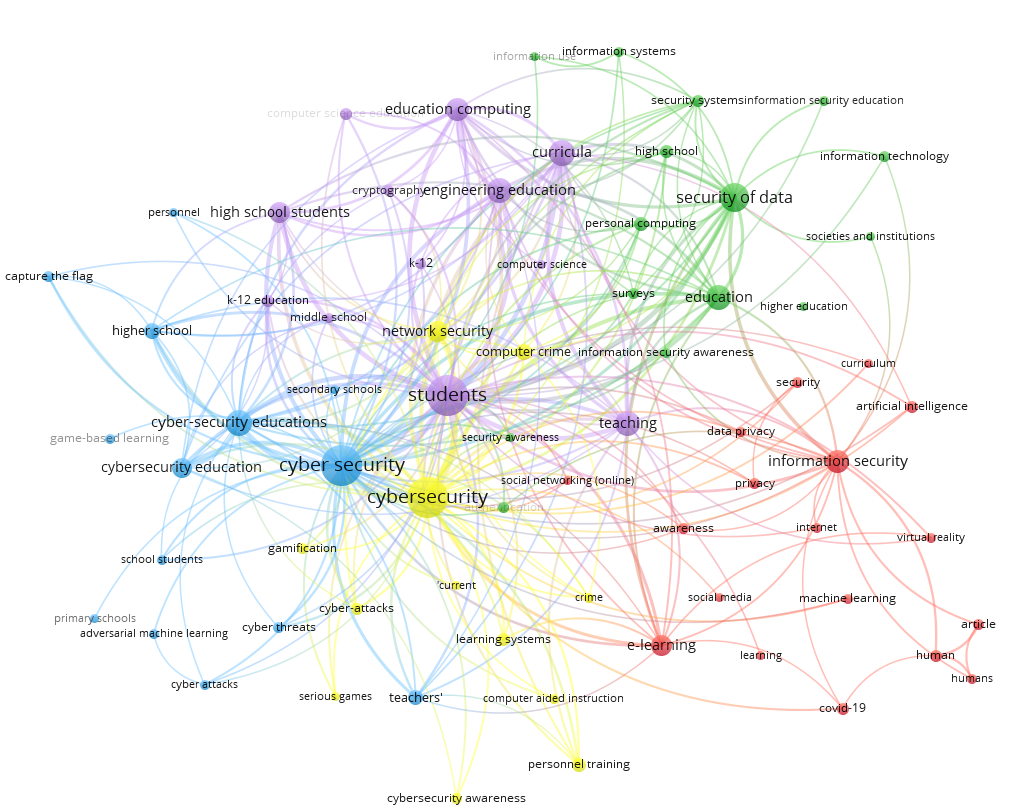
\includegraphics[width=\linewidth]{imgchap1/VOSmap.png}
    \caption{Кластерний аналіз за тематичними напрямами досліджень}
    \label{VOSmap}
\end{figure}

\begin{enumerate}[label=--] % дописать
\item 
\textbf{кластер 1: ``Інформаційні технології та їхній вплив на суспільство''} (червоний) -- об'єднує дослідження, присвячені впливу сучасних технологій на освітній процес та суспільство в цілому. Ключовими термінами є: \textit{artificial intelligence} (середній рік публікації -- 2021.4), \textit{machine learning} (2022.1), \textit{e-learning} (52 появи), \textit{data privacy}, \textit{virtual reality}, \textit{social media}. Високий середній рік публікацій свідчить про актуальність та новизну досліджень у цій сфері;


\item 
\textbf{кластер 2: ``Освіта та обізнаність у сфері інформаційної безпеки''} (зелений) -- наукові праці, що зосереджені на формальній освіті та підвищенні обізнаності в питаннях інформаційної безпеки. Основні терміни: \textit{information security awareness} (45 зв'язків), \textit{information security education} (12 появ), \textit{security of data} (99 появ, 425 зв'язків), \textit{authentication}, \textit{higher education}. Значна кількість зв'язків підкреслює центральну роль цієї тематики в загальному масиві досліджень;

\item 
\textbf{кластер 3: ``Навчання кібербезпеці в освітніх закладах''} (синій) --
найпотужніший кластер за кількістю зв'язків, присвячений практичним аспектам навчання кібербезпеці. Провідні терміни: \textit{cyber security} (195 появ, 1008 зв'язків), \textit{cybersecurity education} (49 появ), \textit{capture the flag}, \textit{game-based learning}. Присутність ігрових методів навчання вказує на інноваційні підходи до викладання кібербезпеки;

\item 
\textbf{кластер 4: ``Тренування та освіта персоналу в галузі кібербезпеки''} (жовтий) --
 охоплює питання професійної підготовки та підвищення кваліфікації. Ключові терміни: \textit{cybersecurity} (195 появ, 862 зв'язки), \textit{computer crime} (середнє цитування -- 14.3), \textit{personnel training}, \textit{serious games}, \textit{gamification}. Високі показники цитування свідчать про значущість тематики в науковій спільноті;

\item 
\textbf{кластер 5: ``Освіта в комп'ютерних науках та інженерії''} (фіолетовий) -- представляє академічні аспекти комп'ютерної освіти. Основні терміни: \textit{curricula} (76 появ), \textit{students} (190 появ, 1008 зв'язків), \textit{computer science education}, \textit{engineering education}, \textit{k-12 education}. Високі показники для терміну ``students'' підкреслюють студентоцентрований підхід у дослідженнях.
\end{enumerate}

Аналіз хронологічного розподілу публікацій виявив, що активне дослідження проблем навчання інформаційній безпеці в закладах загальної середньої освіти розпочалося у 2021--2022 роках. Це пов'язано з масовим переходом на дистанційне навчання під час пандемії COVID-19 та зростанням кіберзагроз в освітньому середовищі.


Сучасні дослідження демонструють зміщення акценту від традиційних методів навчання до інноваційних підходів:

\begin{enumerate}[label=--] % дописать
    \item \textit{гейміфікація освітнього процесу} -- використання ігрових механік для підвищення мотивації та залученості учнів. Терміни ``gamification'', ``serious games'', ``game-based learning'' мають високі показники цитування та актуальності;
    
    \item \textit{змагання CTF (Capture The Flag)} -- практично-орієнтований метод навчання через вирішення реальних задач з кібербезпеки в змагальному форматі. Середній рік публікацій -- 2022.8, що свідчить про новизну підходу;
    
    \item \textit{персоналізоване навчання} -- адаптація освітнього контенту до індивідуальних потреб та рівня підготовки учнів з використанням технологій штучного інтелекту та машинного навчання;
    
    \item \textbf{симуляційне навчання} -- створення безпечного віртуального середовища для відпрацювання навичок протидії кіберзагрозам.
\end{enumerate}


Аналіз зв'язків між кластерами виявив високий рівень міждисциплінарності досліджень. Терміни ``cyber-security educations'' та ``cybersecurity education'' з'являються одночасно в кількох кластерах, що свідчить про інтеграцію технічних, педагогічних та соціальних аспектів проблеми.
На основі проведеного аналізу можна виділити особливості навчання інформаційній безпеці:

\begin{enumerate}[label=--] % дописать
    \item \textit{динамічність предметної області} -- швидка зміна технологій та загроз вимагає постійного оновлення навчальних програм та методичних матеріалів;
    
    \item \textit{обмежена кількість кваліфікованих педагогічних кадрів} -- необхідність підготовки вчителів, які володіють як технічними знаннями, так і педагогічними методиками викладання кібербезпеки;
    
    \item \textit{вікова диференціація} -- необхідність розробки навчальних програм для різних вікових груп;% (primary schools, middle school, high school, k-12);
    
    \item \textbf{практична спрямованість} -- забезпечення балансу між теоретичними знаннями та практичними навичками безпечної поведінки в цифровому середовищі.
\end{enumerate}


Проведений бібліографічний аналіз свідчить про зростання наукового інтересу до проблем навчання учнів інформаційній безпеці. Виявлені тематичні кластери демонструють комплексний характер проблеми, що охоплює технологічні, педагогічні, психологічні та соціальні аспекти.

Домінування термінів ``cyber security'' (195 появ) та ``students'' (190 появ) з найвищими показниками зв'язків підкреслює центральну роль учнівської аудиторії в дослідженнях кібербезпеки. Поява інноваційних методів навчання, таких як гейміфікація, CTF-змагання та симуляційне навчання, свідчить про пошук ефективних педагогічних рішень для формування культури кібербезпеки в молодого покоління.

Перспективними напрямами подальших досліджень є розробка диференційованих методик навчання інформаційній безпеці з урахуванням вікових особливостей учнів, створення інтегрованих навчальних програм, що поєднують технічні та гуманітарні аспекти кібербезпеки, а також підготовка педагогічних кадрів для ефективного викладання цієї дисципліни в закладах загальної середньої освіти.
